\chapter{Newton-Cotes-Formel}



\section{Einleitung und Zielsetzung}

Das Ziel dieser Arbeit ist die wahrscheinlichkeitstheoretische Herleitung und Begründung der Integrationsformeln von Newton-Cotes. Es wird detailliert untersucht, wie Integrale durch eine lineare Kombination von Funktionswerten an äquidistanten Punkten angenähert werden können. Die Güte dieser Annäherung wird anhand der mittleren quadratischen Abweichung gemessen, die ein Maß für die Genauigkeit der Integration darstellt.

\subsection{Theoretische Grundlagen}

In dieser Arbeit wird ein stationärer stochastischer Prozess $\xi(t)$ verwendet, der durch den Erwartungswert $E[\xi(t)] = 0$ und die Varianz $E[\xi^2(t)] = 1$ charakterisiert ist. Der stochastische Prozess dient der Analyse der Fehlerabschätzung und der Bestimmung optimaler Koeffizienten für die Integrationsformeln\textsc{\cite[S. 190]{Newton-Cotes-Formeln}}.

\subsection{Mathematische Herleitung}

Als Mass für die Güte der Näherung wollen wir den Erwartungswert $E[\eta^2]$
benutzen. Bei vorgegebener Korrelationsfunktion ist $h$ und damit auch $E[\eta^2]$
eine Funktion der Schrittweite $h$ und der Koeffizienten $a_i$ Die Formel zur Berechnung der mittleren quadratischen Abweichung
\[
E[\eta^2] = 2 \int_0^{2nh} S(t) dt - 2 \sum_{i = -n}^{+n} a_i \{ S((n + i)h) + S((n-i)h) \} + \sum_{k,i = -n}^{+n} a_k a_i R((i-k)h)
\]
hat das Ziel die Koeffizienten $a_i$ so zu bestimmen, dass der Fehler $E[\eta^2]$ minimiert wird \textsc{\cite[S. 191] {Newton-Cotes-Formeln}}.

\subsection{Minimierung und Ergebnisse}

Es wird gezeigt, dass die minimalen Lösungen der Koeffizienten $a(i)$ den Koeffizienten der Newton-Cotes-Formeln entsprechen. Die Fehlerabschätzungen für diese optimalen Koeffizienten sind vergleichbar mit den Fehlerabschätzungen der Newton-Cotes-Formeln. Eine Taylor-Entwicklung der Koeffizienten bestätigt zudem die Übereinstimmung mit den Newton-Cotes-Koeffizienten.

\section{Versionen von Newton-Cotes}

\subsection{Trapez-Regel}
\label{sec:Trapez}
Die Trapezregel mit der Gewichtung \( [\frac{1}{2} \text{,} \frac{1}{2}] \) \textsc{\cite[S. 342] {Gewichte}} ist durch ihr Intervall auf alle Natürlichen Zahlen anwendbar \textsc{\cite[S. 6] {Trapezregel}}. Die lineare Interpolation an den Intervallenden kann durch
\[  t_{k-1}\] 
bestimmt werden. 
Für die summierte Treapezregel gilt

\[ T(h)=h\cdot(\frac{1}{2} f(a)+f_{t1}+...+f_{t_{n-1}}+\frac{1}{2} f(b)) \text{.}\]

\subsection{Simpson-Regel}
\label{sec:Simpson}
Durch die Gewichtung
\([ \frac{1}{3} \text{,} \frac{4}{3} \text{,}  \frac{1}{3} ]\) mit dem Wert \(n\) = 2
der Simpsonregel wird die numerische Integration über ein Intervall $[a,b]$ approximiert\textsc{\cite[S. 342] {Gewichte}}. Diese Gewichte stammen aus der Quadraturformel für Parabeln und führen zu einer präziseren Näherung im Vergleich zu einfacheren Methoden wie der Trapezregel. Konkret bedeutet dies, dass die Funktion $f(x)$ an den Endpunkten $a$ und $b$ sowie am Mittelpunkt \[{\frac{a + b}{2}} \] evaluiert wird, wobei die Funktionswerte mit den entsprechenden Gewichten multipliziert werden.

Die Simpson-Regel lautet

\begin{equation}
    \label{eq:SimpsonRegel}
    \int_a^b f(x) dx \approx \frac{b - a}{6} [f(a)+4f(\frac{a + b}{2})+f(b)] \text{,}\tag{Simpson Regel}
\end{equation}

wenn ein einfaches Integral \([a, b]\) vorliegt\textsc{\cite[S. 17] {Simpsonregel/Milneregel}}.

\subsection{\(\frac{3}{8}\)-Regel}
\label{sec:3/8}
Die \(\frac{3}{8}\)-Regel mit der Gewichtung \( [\frac{3}{8} \text{,}\frac{9}{8} \text{,}\frac{9}{8} \text{,}\frac{3}{8}]\), dem gekürzten Wert $n$ = 3 \textsc{\cite[S. 342] {Gewichte}} und der Form

\[ \int_a^b f(x) dx \approx (b-a) [w_0f_0 + w_1f_1 + w_2f_2 + w_3f_3]\]

wird angewendet, indem das Intervall $[a, b]$ in $n$ Teilintervalle geteilt wird, wobei $n$ ein Vielfaches von 3 sein muss.

\subsection{Milne-Regel}
\label{sec:Milne}
Die Milne-Regel mit der Gewichtung \( [\frac{7}{90} \text{,} \frac{32}{90} \text{,} \frac{12}{90} \text{,} \frac{32}{90} \text{,} \frac{7}{90}] \) \textsc{\cite[S. 342] {Gewichte}}
erhält man durch die Formel
\[ \int_a^b f(x) dx \approx \frac{b - a}{90} \cdot (7f(x_0) + 32f(x_1) + 12f(x_2) + 32f(x_3) + 7f(x_4))\]
\textsc{\cite[S. 19] {Simpsonregel/Milneregel}}.

\subsection{Weddle-Regel}
\label{sec:Weddle}
Die Weddle-Regel mit der Gewichtung \( [\frac{41}{840} \text{,} \frac{216}{840} \text{,} \frac{27}{840} \text{,} \frac{272}{840} \text{,} \frac{27}{840} \text{,} \frac{216}{840} \text{,} \frac{41}{840}] \) \textsc{\cite[S. 342] {Gewichte}} mit der Formel
\[ Q_a^b (f) := (b - a) \sum_{i=0}^{n0} \sigma_i f(x_i)\] 

\textsc{\cite[S. 5] {Weddleregel}} erzeugt den Fehler \[ \frac{9}{1400}h^9f^{(9)} (\hat{x}) \text{.} \]


%%%%%%%%%%%%%%%%%%%%%%%%%%%%%%%%%%%%%%%%%%%%%%%%%%%%%%%%%%%%%%%%%%%%%%%%%%%%%%%%%%%%%%%%%%%%%%%%%%%%%%%%%%%%%%%%%%%%%%%%%%%%%%%%%%%%%%%%%%%%%%%%%%%%%%%%%%
%%%%%%%%%%%%%%%%%%%%%%%%%%%%%%%%%%%%%%%%%%%%%%%%%%%%%%%%%%%%%%%%%%%%%%%%%%%%%%%%%%%%%%%%%%%%%%%%%%%%%%%%%%%%%%%%%%%%%%%%%%%%%%%%%%%%%%%%%%%%%%%%%%%%%%%%%%
%%%%%%%%%%%%%%%%%% Simpson-Formel, Varianten sowie Unterschiede und wo welche Simpson Formel sinnvoll ist %%%%%%%%%%%%%%%%%%%%%%%%%%%%%%%%%%%%%%%%%%%%%%%%

\section{Simpson-Formel, Varianten sowie Unterschiede und wo welche Simpson Formel sinnvoll ist}

\subsection{Varianten}

Bei der Simpson Regel gibt es vier verschiedene Varianten, welche nochmal in zwei Kategorien aufgeilt werden können. Man kann es in die \(\frac{1}{3}\)-Formeln und die \(\frac{3}{8}\)-Formeln unterteilen. Diese kann man dann wiederrum in die Einfache Simpson-\(\frac{1}{3}\)-Formel und die Zusammengesetzte Simpson-\(\frac{1}{3}\)-Formel, sowie die Einfache-\(\frac{3}{8}\)-Formel und die Zusammengesetzte Simpson-\(\frac{3}{8}\)-Formel unterteilen \textsc{\cite[S. 342]{SimpsonVarianten}}  \textsc{\cite[S. 327]{BasicNumMath}}.


\subsection{Unterschiede}\label{sec:Unterschiede}

Bei den Unterschieden kann man ebenfalls wieder in die zwei Kategorien \(\frac{1}{3}\)-Formel und \(\frac{3}{8}\)-Formel unterteilen. Die Einfache Simpson-\(\frac{1}{3}\)-Formel kann man für ein einzelnes Intervall benutzen, welches in zwei gleich große Teile geteilt wurde. Die Zusammengesetzte Simpson-\(\frac{1}{3}\)-Formel kann man dahingegen für ein Intervall nutzen, welches in mehrere gleich große Teile geteilt wurde, wobei die Anzahl durch zwei teilbar sein muss. Bei den \(\frac{3}{8}\)-Formeln ist das so ähnlich, bis auf enen kleinen Unterschied. Die Einfache-\(\frac{3}{8}\)-Formel nutzt man für ein einzelnes Intervall, welches in drei gleich große Teile geteilt wurde und die Zusammengesetzte Simpson-\(\frac{3}{8}\)-Formel nutzt man für ein Intervall, das in mehrere gleich große Teile geteilt wurde, allerdings muss die Anzahl der Teile hierbei durch drei teilbar sein \textsc{\cite[S. 310]{NumMathe}} \textsc{\cite[S. 180]{NumMethodsScienceEng}}.


\subsection{Unter welchen Bedingungen bzw. Anforderungen ist welche Simpson Formel sinnvoll}

Im allgemeinen dienen die Simpson-Formeln dazu, eine höhere Genauigkeit zu erreichen als beispielsweise mit der Rechtecks- oder Trapezberechnung. \textsc{\cite[S. 310]{NumMathe}} Sofern die Abstände der Punkte gleichmäßig sind, kann man Formeln, wie die Simpson-Formeln, höherer Ordnung anwenden. Sowohl die \(\frac{1}{3}\)-Formel und die \(\frac{3}{8}\)-Formel haben die gleiche Genauigkeit. Man kann die Simpson-Formeln allerdings nicht nutzen, wenn die Punkte nicht gleichmäßig vertielt sind \textsc{\cite[S. 186]{NumMethodsScienceEng}}. Wie bei den Unterschieden \ref{Unterschiede} erwähnt, kann man die \(\frac{1}{3}\)-Formel dafür benutzen, um eine Fläche in einem Intervall zu berechnen, welche aus einer geraden Anzahl von Teilintervallen besteht. Hierbei muss man allerdings darauf achten, dass die Einfache Simpson-\(\frac{1}{3}\)-Formel nur zwei Teilintervalle haben darf, dafür aber die Zusammengesetzte Simpson-\(\frac{1}{3}\)-Formel aus mehreren Teilintervallen bestehen darf, diese Anzahl aber durch zwei teilbar sein muss. Bei der \(\frac{3}{8}\)-Formel ist das ähnlich, nur das man nicht die Zahl zwei nimmt sondern drei. Die Einfache Simpson-\(\frac{3}{8}\)-Formel muss aus drei Teilintervallen bestehen und die Zusammengesetzte Simpson-\(\frac{3}{8}\)-Formel muss aus einer Anzahl an Teilintervallen bestehen, welche durch drei teilbar ist \textsc{\cite[S. 180]{NumMethodsScienceEng}} \textsc{\cite[S. 186]{NumMethodsScienceEng}}. 

\section{Implementation der Newton-Cotes-Formeln in Python}

\subsection{Vorgehen}
Die Approximation der Integration mit den Newton-Cotes-Formeln soll nun per Code näher betrachtet werden. Hierzu werden, wie in \ref{sec:ImplFDM}, die Python-libraries \texttt{Numpy} und \texttt{Matplotlib} verwendet.

Das Verfahren wird anhand der Schnittgrößen aus der Technischen Mechanik erklärt. Das Beispiel (\ref{fig:ExampleInternalForce})\footnote{Entnommen aus \href{https://pickedshares.com/technische-mechanik-2-uebung-10-traeger-mit-dreieckfoermiger-streckenlast/}{https://pickedshares.com/technische-mechanik-2-uebung-10-traeger-mit-dreieckfoermiger-streckenlast/}} bildet einen, durch eine Linienlast $q_0$ belasteter Träger, welcher an einer Einspannung $A$ gelagert wurde. Der Träger hat die Länge $l$. Es wird ein Koordinatensystem angelegt, mit der horizontalen $x$-Achse, welche nach rechts positiv ist und die vertikale $z$-Achse, welche nach unten positiv ist. Der Ursprung des Koordinatensystems liegt im Lager $A$.

\begin{figure}[h]
    \centering
    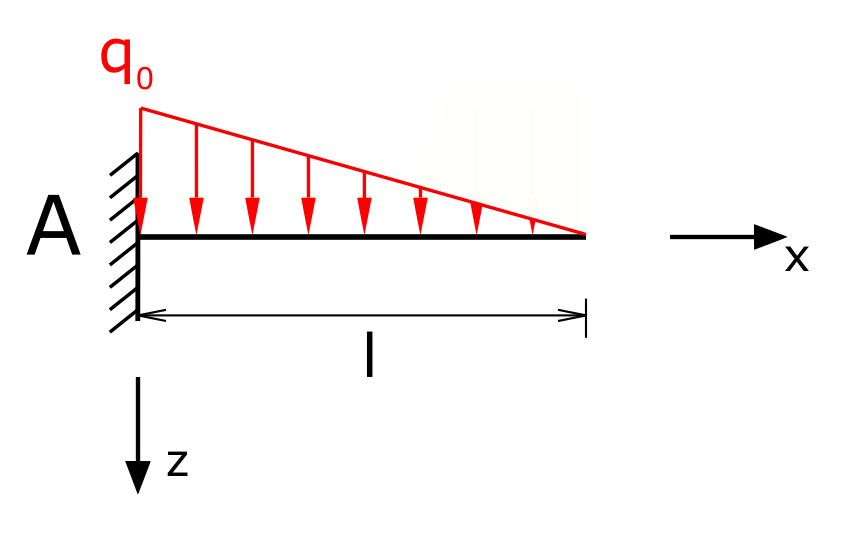
\includegraphics[scale = 0.5]{images/example_internal_force.png}
    \caption{Träger an einem Festlager mit Länge $l$ und Streckenlast $q_0$}
    \label{fig:ExampleInternalForce}
\end{figure}

\subsection{Aus Streckenlast zur Querkraft und Moment}
 Ziel ist es den Querkraft- und Momentenverlauf als Graphen darzustellen. Dazu werden die verschiedenen Varianten der Newton-Cotes-Formeln(NCF), um das Integral zu approximieren, verwendet, welche im Verlauf der Implementierung erläutert werden.

Zur Darstellung der Graphen werden Zahlenbeispiele für die konstanten Größen verwendet. Es wird angemommen, die Länge des Trägers $l$ sei 10 Meter und die Streckenlast $q_0$ entspreche 2 Newton pro Meter.

Der lineare Verlauf lässt sich durch die Gleichung

\begin{equation}
    \label{eq:Streckenlast}
    q(x) = \frac{q_0 (l - x)}{l}\tag{eq1}
\end{equation}

ermitteln. 
Der Querkraft- und Momentverlauf lassen sich dann durch

\begin{equation}
    \label{eq:Querkraft}
    Q(x) = - \int q(x) dx\tag{eq2}
\end{equation}

und

\begin{equation}
    \label{eq:Moment}
    M(x) = \int Q(x) dx\tag{eq3}
\end{equation}

errechnen.

\subsection{Python-Code für die \texttt{NewtonCotes}- und \texttt{SimpsonRule}-Klasse}
Nun werden die \texttt{NewtonCotes}- und \texttt{SimpsonRule}-Klasse näher betrachtet.

\paragraph{Code der \texttt{NewtonCotes}-Klasse}

Die \texttt{NewtonCotes}-Klasse bietet Methoden zur numerischen Berechnung von Integralen mittels der NCF. Es beinhaltet nur die ersten vier Formeln, also von \ref{sec:Trapez} bis \ref{sec:Milne}. Hier ist der vollständige Python-Code:

\begin{lstlisting}[language=Python, caption={Vollständiger Code der NewtonCotes-Klasse}, label={lst:NewtonCotesClass}]
    from typing import Callable
    import numpy as np
    
    class NewtonCotes:
        weightOptions = [
            np.array([1, 1]) * 1 / 2,  #trapezoidal rule
            np.array([1, 4, 1]) * 1 / 3,  #simpson rule
            np.array([1, 3, 3, 1]) * 3 / 8,  #3/8 rule
            np.array([7, 32, 12, 32, 7]) * 2 / 45,  #milne rule
        ]
    
        def __init__(self, n: int):
            assert 0 < n < 5 and isinstance(n, int)
            self.n = n
            self.weight = self.weightOptions[n - 1]
    
        def calculate_integral(
             self,
             f: Callable[[float], float],
             a: float,
             b: float
            ) -> float:
            A = 0
            h = (b - a) / self.n
            for i in range(self.n + 1):
                xi = a + i * h
                A += self.weight[i] * f(xi)
            A *= h
            return A
\end{lstlisting}

\paragraph{Code der \texttt{SimpsonRule}-Klasse}

Die \texttt{SimpsonRule}-Klasse ist eine spezielle Unterklasse der \texttt{NewtonCotes}-Klasse, die die Simpson-Regel zur numerischen Integration verwendet. Hier ist der vollständige Python-Code:

\begin{lstlisting}[language=Python, caption={Vollständiger Code der SimpsonRule-Klasse}, label={lst:SimpsonRuleClass}]
from typing import Callable
import numpy as np
from Code.Approximation_Integral
        .Newton_Cotes.NewtonCotes import NewtonCotes

class SimpsonRule(NewtonCotes):
    def __init__(self, node_count=10):
        super().__init__(2)
        assert node_count > 0
        assert node_count % 2 == 0
        self.node_count = node_count

    def calculate_integral_composite(
         self,
         f: Callable[[float], float],
         a: float,
         b: float
        ) -> float:
        h = (b - a) / self.node_count
        A = f(a) + f(b)
        for i in range(1, self.node_count):
            xi = a + i * h
            if i % 2 == 0:
                A += 2 * f(xi)
            else:
                A += 4 * f(xi)
        return A * h / 3

    def calculate_integral_simple(
         self,
         f: Callable[[float], float],
         a: float,
         b: float
        ) -> float:
        h = (b - a) / 6
        return h * (f(a) + f(b) + 4 * f((a + b)/2))
\end{lstlisting}

\subsection{Erklärung der Klassen und deren Methoden}

\paragraph{\texttt{NewtonCotes}-Klasse}
Das Attribut \texttt{weightOptions} zeigt die verschiedenen Gewichte der NCF. Das Gewicht \texttt{weight}, welches zur Berechnung des Integrals benutzt wird, wird durch die Anzahl an Knoten bestimmt.

Passend dazu ist die Methode \texttt{\_\_init\_\_} der Konstruktor des Objekts, der die Anzahl an Knoten \texttt{n} als Parameter annimmt. Der Code beinhaltet nur die ersten vier Formeln, deshalb kann \texttt{n} maximal 4 sein.

Die Methode \texttt{calculate\_integral} ermittelt die Fläche zwischen einer Funktion \texttt{f} und der $x$-Achse im Intervall \texttt{[a, b]}.

\paragraph{Parameter:}
\begin{itemize}
    \item \texttt{f}: Der Integrant, der eine Funktion ist. Diese sollte einen \texttt{float}-Wert annehmen und sowohl zurückgeben.
    \item \texttt{a}: ein \texttt{float}, der die untere Grenze des Intervalls angibt
    \item \texttt{b}: ein \texttt{float}, der die obere Grenze des Intervalls angibt
\end{itemize}

\paragraph{Rückgabewert:}
\begin{itemize}
    \item \texttt{float}: Die resultierende Fläche
\end{itemize}

\paragraph{Funktionsweise:}
Der Algorithmus bestimmt für jedes iterierte $x_i$, welches die Stellen der einzelnen Knoten sind, den Funktionswert und multipliziert diesen mit dem jeweiligen Gewicht. Alle auf dieser Weise ermittelten Werte werden summiert und mit dem Abstand zwischen den einzelnen Knoten \texttt{h} multipliziert.

\paragraph{\texttt{SimpsonRule}-Klasse}
Die \texttt{SimpsonRule}-Klasse vererbt die \texttt{NewtonCotes}-Klasse. Dadurch wird im Konstruktor der \texttt{SimpsonRule}-Klasse die Superklasse aufgerufen mit dem Parameter \texttt{n=2}, da diese der Simpson-Regel entspricht. Der Konstruktor von dieser Klasse besitzt einen optionalen Parameter \texttt{node\_count}, der standarmäßig auf $10$ gesetzt wird. Dieser beschreibt die Anzahl der Knoten, die benutzt werden, um das Integral zu approximieren. Die Anzahl muss gerade sein, wie in \ref{sec:Unterschiede} schon erwähnt wurde.

Die \texttt{calculate\_integral\_composite}-Methode kann stetig zusammengesetzte Intervalle benutzen, das heißt es ist abhängig vom Attribut \texttt{node\_count}, um das Integral anzunähern.

\paragraph{Parameter und Rückgabewert}
Diese können analog aus der \texttt{calculate\_integral}-Methode der Superklasse\texttt{NewtonCotes} entnommen werden.

\paragraph{Funktionsweise:}
Die Funktionswerte an den Randstellen von $x$ haben keine Gewichtung. Für jedes gerade $x_i$ wird der Funktionswert an dieser Stelle mit der Gewichtung $\frac{2}{3}$ und jedes ungerade mit $\frac{4}{3}$ multipliziert. Diese Werte werden miteinander addiert und mit dem Abstand \texttt{h} multipliziert.

Die \texttt{calculate\_integral\_simple}-Methode approximiert das Integral nur für ein einfaches Intervall \texttt{[a, b]}, das heißt es ist nicht abhängig von \texttt{node\_count}.

\paragraph{Parameter und Rückgabewert}
Diese können analog aus der \texttt{calculate\_integral}-Methode der Superklasse\texttt{NewtonCotes} entnommen werden.

\paragraph{Funktionsweise:}
Die Formel aus \ref{eq:SimpsonRegel} wird übernommen und die Fläche wird zurückgegeben.

\subsection{Anwendung der Newton-Cotes-Formeln zur Bestimmung der Schnittgrößen}

Zunächst wird die \texttt{InternalForces}-Klasse näher betrachtet, die zur Veranschaulichung des Beispiels eines gelagerten Trägers(Abbildung: \ref{fig:ExampleInternalForce}) und die Verwendung der zuvor erwähnten Klassen \texttt{NewtonCotes}(\ref{lst:NewtonCotesClass}) und \texttt{SimpsonRule}(\ref{lst:SimpsonRuleClass}).

Zur Bestimmung der Schnittgrößen (Querkraft $Q(x)$ und Moment $M(x)$) des belasteten Trägers werden die oben implementierten Klassen verwendet und die Konstanten $q_0$ und $l$ eingeführt. Es wird ein Objekt der Klasse \texttt{NewtonCotes} erstellt mit dem Parameter für \texttt{n = 3}. Dies entspricht der $\frac{3}{8}$-Regel. Zusätzlich wird ein Objekt der Klasse \texttt{SimpsonRule} mit dem optionalen Parameter \texttt{node\_count=100}, für eine bessere Approxmierung des Integrals.

\begin{lstlisting}[language=Python]
    import numpy as np
    import matplotlib.pyplot as plt
    from Code.Approximation_Integral
            .Newton_Cotes.SimpsonRule import SimpsonRule
    from Code.Approximation_Integral
            .Newton_Cotes.NewtonCotes import NewtonCotes
    
    l = 10  #Meter
    q_0 = 2  #Newton/Meter
    newtonCotes = NewtonCotes(3)
    simpson = SimpsonRule(node_count=100)
\end{lstlisting}

Es wird die Funktion für die Streckenlast \texttt{q(x)}, welche analog zur Formel für $q(x)$ aus \ref{eq:Streckenlast} implementiert wurde, erstellt.
Für die Querkraft \texttt{Q(x)} wird nach \ref{eq:Querkraft} das negative Integral von \texttt{q(x)} und das Integral davon für das Moment \texttt{M(x)} nach \ref{eq:Moment}.

\begin{lstlisting}[language=Python, label={lst:Func}]
    def q(x: float) -> float:
        return (q_0 * (l - x)) / l
    
    
    def Q(x: float) -> float:
        return -1 * simpson.calculate_integral_composite(q, x, l)
    
    
    def M(x: float) -> float:
        return simpson.calculate_integral_simple(Q, x, l)
\end{lstlisting}

In der Methode \texttt{single\_value\_integral} wird die $\frac{3}{8}$ - Regel aus \ref{lst:NewtonCotesClass} zur Berechnung der Querkraft $Q(x)$ mithilfe des Integrals von der Streckenlast $q(x)$ im Intervall 0 bis 5 benutzt. Diese Methode zeigt, die Annäherung des Integrals und den tatsächlichen, wenn man das zuvor ausgerechnete Integral benutzt.

\begin{lstlisting}[language=Python]
    def single_value_integral():
        integral_with_trapezoidal = newtonCotes.calculate_integral(q, 0, 5)
        approximated_result = (((q_0 * l) / 4) - integral_with_trapezoidal)
        print(f"Approx: {approximated_result}")
        print(f"Tatsaechlich: {Q(5) - Q(0)}")
\end{lstlisting}

Die vollständige Ausgabe, die hier aus Platzgründen(Formaierung) nicht angezeigt wurde, sieht so aus:

\begin{lstlisting}[language=Python]
Console:
    Angenaehertes Integral bei Q(5) - Q(0) mit Trapezregel: 7.5 N
    Tatsaechliches Integral bei Q(5) - Q(0): 7.5 N
\end{lstlisting}

Anschließend wird der ganze Verlauf der Schnittgrößen als drei Graphen mithilfe von \texttt{Matplotlib} in der Methode \texttt{plot\_internal\_forces}. Es wird ein \texttt{Numpy}-Array für \texttt{x} von \texttt{0} bis \texttt{l} erstellt, also den Verlauf von $x$ über das Tragwerk mit der Länge $l$. Die einzelnen Werte der Funktionen werden mit den vorherig erläuterten Methoden (\ref{lst:Func}) berechnet. Die einzelnen Funktionen werden schließlich geplottet.

\begin{lstlisting}
    def plot_internal_forces():
        x = np.linspace(0, l, 100)
    
        q_values = np.array([q(i) for i in x])
        Q_values = np.array([Q(i) for i in x])
        M_values = np.array([M(i) for i in x])
    
        fig, (ax1, ax2, ax3) = plt.subplots(3, 1, figsize=(10, 6))
    
        ax1.plot(x, q_values, label=r'Streckenlast $q(x)$', color='r')
        ax1.set_ylabel(r'$q (N/M)$')
        ax1.fill_between(x, q_values,
                color='red', alpha=0.2, label=r'$\int q(x) dx$')
        ax1.legend()
        ax1.grid()
    
        ax2.plot(x, Q_values, label=r'Querkraftverlauf $Q(x)$', color='r')
        ax2.set_ylabel(r'$Q (N)$')
        ax2.fill_between(x, Q_values,
                color='red', alpha=0.2, label=r'$\int Q(x) dx$')
        ax2.legend()
        ax2.grid()
    
        ax3.plot(x, M_values, label=r'Momentverlauf $M(x)$', color='r')
        ax3.set_xlabel(r'$x (m)$')
        ax3.set_ylabel(r'$M (Nm)$')
        ax3.fill_between(x, M_values,
                color='red', alpha=0.2, label=r'$\int M(x) dx$')
        ax3.legend()
        ax3.grid()
    
        plt.tight_layout()
        plt.show()
\end{lstlisting}

Schließlich werden die zwei Funktionen aufgerufen und es entsteht das Bild aus Abbildung (\ref{fig:InternalForcesPlot})

\begin{lstlisting}[language=Python]
    single_value_integral()
    plot_internal_forces()
\end{lstlisting}

\begin{figure}[h]
    \centering
    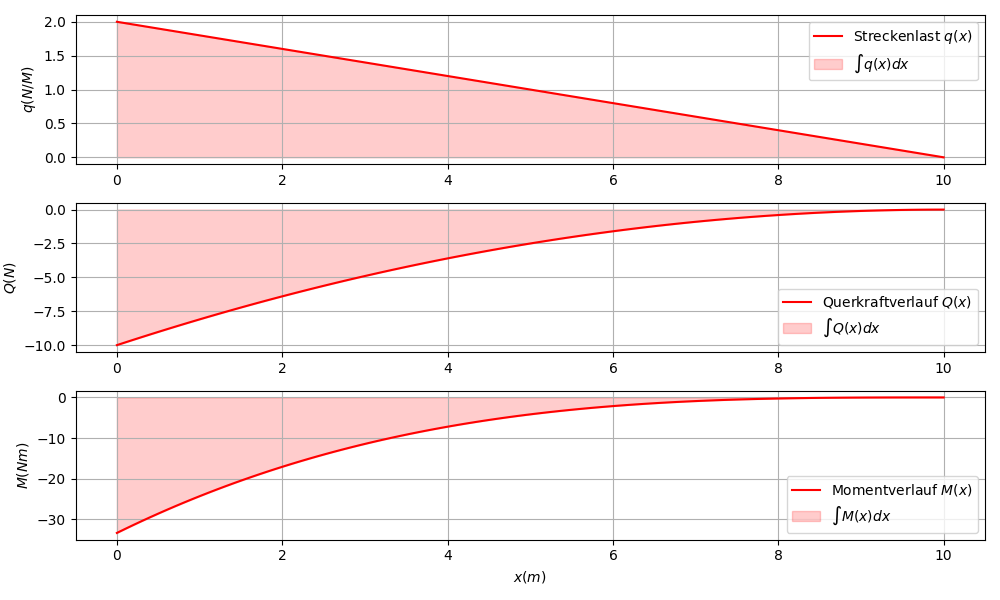
\includegraphics[width=\textwidth]{images/internal_forces_plot.png}
    \caption{Graphen für $q(x)$ in $\frac{N}{m}$, $Q(x)$ in $N$ und $M(x)$ in $Nm$ für $q_0=2, l=10$}
    \label{fig:InternalForcesPlot}
\end{figure}

\subsection{Fazit}
Die dargestellten Graphen (\ref{fig:InternalForcesPlot}) zeigen den Verlauf der Streckenlast $q(x)$, der Querkraft $Q(x)$ und des Moments $M(x)$ entlang eines Trägers mit einer Länge von $l = 10$ Metern und einer linear verteilten Streckenlast von $q_0 = 2$ Newton pro Meter. 

Die Analyse des Verhaltens eines Trägers unter linear abnehmender Streckenlast ist ein klassisches Problem in der Bauingenieurwissenschaft und bietet wertvolle Einblicke in die Tragwerksdynamik. Man erkennt, dass die Streckenlast $q(x)$, die linear von $q_0$ auf null am Ende des Trägers abfällt, zu einer Querkraft $Q(x)$ führt, die eine quadratische Abhängigkeit zeigt, und zu einem Biegemoment $M(x)$ , das kubisch mit $x$ ansteigt.

Die Ergebnisse zeigen, wie die Kräfte entlang des Trägers verlaufen. Die Querkraft beginnt bei $x=0$ mit dem Maximum und fällt zum Ende hin ab, was darauf hindeutet, dass der Träger an seinem fest geschweißten Ende die größte Belastung erfährt. Das Moment hat einen kubischen Verlauf, der vom maximalen Moment gegen null läuft, was die zunehmende Biegung des Trägers unter der Last verdeutlicht.

Die numerische Integration, also durch die Newton-Cotes-Formeln, hlft diese Verläufe anzunähern und per Code zu analysieren, wenn Zurückgreifen auf analoge Methoden nicht praktikabel ist. Dies ist besonders nützlich in komplizierten realen Anwendungsfällen, wo Lastverteilungen variieren oder nicht standardmäßige Geometrien eine Rolle spielen.